\chapter{Refleksie oor Projekmylpale}

\section{Inleiding}

Hierdie hoofstuk gee 'n oorsig van die projekmylpale en die tydsraamwerk wat
gevolg is tydens die ontwikkeling van die sagtewarestelsel. Dit sluit 'n
bespreking in van die oorspronklike Gantt-grafiek wat gebruik is om die projek se vordering te
monitor en te bestuur, asook 'n opgedateerde weergawe van die Gantt-grafiek wat die
werklike vordering en enige aanpassings aan die tydsraamwerk aandui.

\section{Gantt-grafiek}
\begin{figure}[htbp]
    \centering
    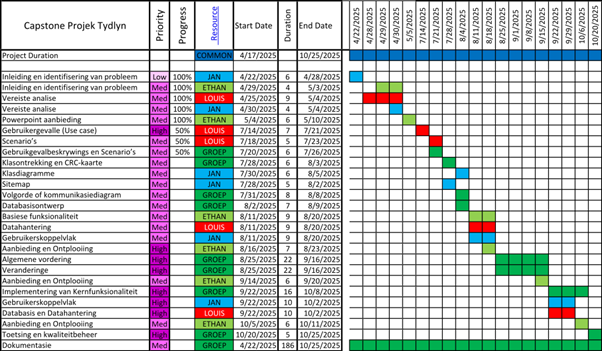
\includegraphics[width=\textwidth]{figures/gantt-grafiek.png}
    \caption{Gantt-grafiek vir projektydsraamwerk en mylpale}
    \label{fig:gantt_chart_again}
\end{figure}

\begin{figure}[htbp]
    \centering
    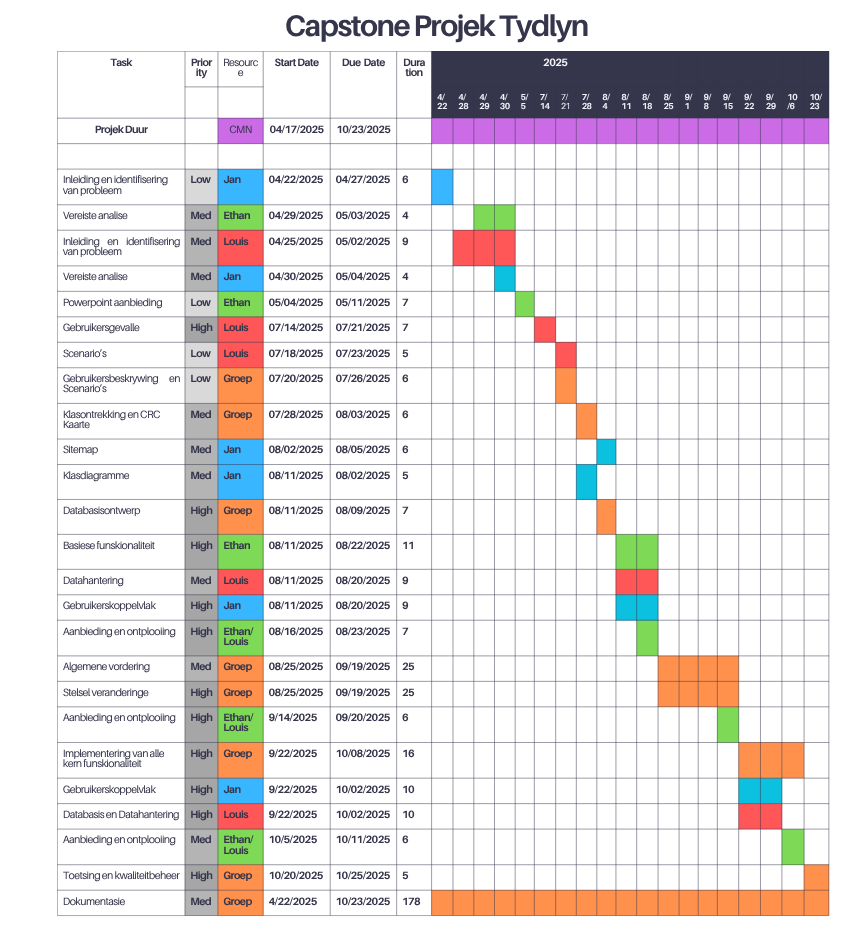
\includegraphics[width=\textwidth]{figures/gantt2.png}
    \caption{Opgedateerde Gantt-grafiek vir projektydsraamwerk en mylpale}
    \label{fig:gantt_chart_2}
\end{figure}

Die opgedateerde Gantt-grafiek in Figuur \ref{fig:gantt_chart_2} weerspieël die
werklike vordering van die projek en enige aanpassings wat gemaak is aan die
oorspronklike tydsraamwerk. Dit toon die voltooiing van verskeie mylpale,
insluitend die voltooiing van kernfunksies, toetsing, en uiteindelike ontplooing
van die stelsel. Enige vertragings of verskuiwings in die tydsraamwerk is ook
aangedui, saam met die redes daarvoor. 

Die eerste groot verandering wat opgemerk
sal word is die aanpassing van die finale aanbiedingsdatum na die 23ste Oktober,
wat ooreenstem met die opgedateerde projekkalender van die Akademia. Verder is
sekere sleutel aktiviteite soos \textit{Basiese funksies geïmplementeer} en \textit{Toetsing
voltooi} as hoë prioriteit gemerk, om die belangrikheid daarvan in die
projeklewensiklus te beklemtoon. 'n Paar ander datums is aangepas om die werklike vordering van die span beter te weerspieël.

\section{Gevolgtrekking}

Die projek het oor die loop van die semester verskeie mylpale bereik, soos
aangedui in die Gantt-grafieke. Terwyl die oorspronklike tydsraamwerk 'n nuttige
riglyn verskaf het, was daar aanpassings nodig om onvoorsiene uitdagings en
veranderende vereistes te hanteer. Die opgedateerde Gantt-grafiek weerspieël
hierdie aanpassings en toon die span se vermoë om effektief te beplan en aan te
pas gedurende die projeklewensiklus. Verder is 'n eenvoudiger templaat gebruik om die Gantt-grafiek te genereer, wat die proses van opdatering en aanpassing vergemaklik het.

\chapter{Reflektiewe Leer en Profesionele Ontwikkeling}

\section{Inleiding}
Hierdie hoofstuk gee 'n refleksie oor die span se dinamika, tydsbestuur, koderingstandaarde, toetsingstrategieë, tegnologie- en argitektuurkeuses, sowel as die algehele voldoening van projekvereistes. Dit bespreek ook die kommunikasie met die studieleier, terugvoermeganismes, en die produksie-gereedheid van die stelsel. Laastens bied dit 'n evaluering van die span se prestasie en identifiseer areas vir verbetering in toekomstige projekte.

\section{Spandinamika en Samewerking}

Ons span het vroeg in die lewensiklus van die projek rolle opgestel. Elke rol
het duidelike take gehad waaraan aandag gegee moes word. Elke rol was so geskep
sodat spanlede gelyk bygedra kan volgens hul portefeulje beskrywing.

Louis was die spanleier, en was verantwoordelik vir die reël en
bestuur van vergaderings. Verder was hy verantwoordelik vir die organisasie
van take. Hy het ook die databasis en bediener-kant ontwerp en
geimpliminteer. Verder het hy die sekuriteit van die stelsel bestuur en die
ontplooing van die stelsel hanteer.

Jan was die UI/UX ontwerper. Hy was verantwoordelik vir die oorspronklike uitleg
van skerms, en die verfyning van die algehele ontwerp van die stelsel. Hy
het ook van die skerms geïntegreer in die stelsel. Hy het ook toetsing aan die gebruikerkant gedoen.

Ethan was die hoof ontwikkelaar op die kliënte-kant en mobiele toepassing.
Hy het Jan se skerm ontwerpe geïmplementeer en sorgvuldig dit getoets. Hy het
ook van die gebruikerservaring van sommige komponente verbeter. Hy het die
ontwerp van logos, voorblaaie, demonstrasies en aanbiedings gedoen.

Die span het via Discord en Whatsapp gekomunikeer. Verder het ons vergaderings
op kampus gehou. Dit het effektief gewerk vir ons en was voldoende vir die skaal
van die projek.

Die span het nie enige groot konflikte gehad om te hanteer nie, elke spanlid
was oop vir nuwe idees en het goed saamgewerk. Klien meningsverskille is
goed hanteer, deur ooplik te kommunikeer en kompromieë te maak waar nodig.
Die enkele konflikte wat ontstaan het waar daar nie 'n duidelike oplossing was
nie, het die spanleier die finale besluit geneem nadat alle menings oorweeg is.

Verantwoordbaarheid was deur sperdatums en meilpale vir ontwikkeling vir elke
week te stel, en deurlopend probeer daarby te hou. Ons het 'n kultuur van 
verantwoordbaarheid geskep waar elke spanlid hul take ernstig opgeneem het, maar
ook nie bang was om hulp te vra as dit nodig was nie.

Ons span se moraal was algeheel goed deurlopend. Ons het nie enige groot
probleme ervaar wat die moraal negatief beïnvloed het nie. Ons het mekaar
ondersteun en gemotiveer om die projek suksesvol af te handel.

\section{Projekbestuur en Prosesse}

Ons tydlyn was algeheel realisties, ons het goed ons kapasiteit benut. Van die vertragings was as gevolg van die onderskatting van die kompleksiteit van sommige oplossings, maar dit was effektief bestuur deur om vroegtydig die probleme te kommunikeer en saam te werk.

Ons het 'n vaste bestaande metodologie gevolg nie, maar ons het baie inspirasie
by Agile geneem. Ons het elke week met mekaar ingeskakel om seker te maak dat
almal se werk op spoor is, verder het ons take volgens ons kapasiteit ingedeel
op 'n weeklikse basis. Dit was baie effektief vir ons span, omdat dit vryheid
gegee het om take te kies, maar steeds die nodige struktuur en verantwoordelikheid gehandhaaf het.

Vir taakopvolging het ons 'n kanaal op Discord geskep vir taakuitdeling en
bestuur. Elke vergadering het die spanleier take op die kanaal gestuur, en
spanlede het hul vordering op die take gedeel. Dit was voldoendoende vir die
skaal van die projek, en ons het geen uitdagings daarmee ervaar nie.

Die kere waar daar onverwagte probleme of veranderinge aan vereistes was, het ons besluit volgens ons kapasiteit hoe ons die nuwe funksies gaan indeel vir spanlede. Omdat ons taakverdeling en tydsbestuur effektief was, kon ons maklik veranderinge inwerk.

Ons spanvergaderings was naby altyd produktief. Ons het vinnig en by die punt
uitgekom en gehou. Ons het ook refleksie sessies onmiddelik na elke vergadering
met ons studieleier en aanbiedings gehou, waar ons terugvoer kon bespreek. As
ons 'n aspek van ons vergaderings moes verbeter, sou ons sorg dat ons meer tyd
toegeken het aan in diepte bespreking van ontwikkeling van die kern funksies,
voordat ons met implementasie daarvan begin het. Ons het wel vinnig die aspek
intern aangespreek en verbeter.

\section{Tegniese Samewerking}

Vir kodebustuur het ons 5 git bewaarplekke (repositories) geskep. Een vir ons
bediener-kant en een vir ons kliënt-kant. Verder het ons een vir ons
dokumentasie geskep, een vir ons ontplooing op 'n Kubernetes kluster, en een vir
ons OCI demonstrasie. 

Nuwe ontwikkeling was deur funksie takke (feature branches) hanteer, en in te
voeg soos voltooi deur trek versoeke (pull requests).

Ons het 'n konsekwente koderun standaard gefokus op produksie-gerede kode
gehandhaaf, en ons dokumentasie was deurlopend op datum gehou.

Ons het gebruik gemaak van handmatige toetsing vir die eerste fases van die
implementasie. Eenheids- en integrasietoetse vir bediener-kant was geskep en
gebruikerskoppelvlaktoetsing was handmatig gedoen.

Ons het tegnologie en argitektuur gekies volgens ervaring en relevansie tot 'n
moderne produksie-omgewing. Ons het 'n PWA benadering gevolg met React en
Typescript op die kliënt-kant, en Spring met Java op die bediener-kant. Postgres
is gebruik as die databasis, en Docker en Kubernetes is gebruik vir ontplooing.
NGINX is gebruik as die omgekeerde-voorportaal (reverse proxy) en
laai-balansering (load balancing). NGINX het ook die statiese lêers van die
kliënt-kant hanteer. 

Om kennisdeling en leer te bevorder het ons vergaderings gehou waar ons met
mekaar gesels het oor ons gekose tegnologie en wat die hoof probleme was wat
sekere pakete oplos is. Verder het ons oor die belangrikste aspekte van 'n
tegnologie bespreek voor dit gebruik word, asook eie kennis en navorsing soos
nodig gebruik gedoen om die tegnologie effektief te implementeer.

\section{Projekuitkomste}

Ons projek het verseker aan die oorspronklike doelwitte en vereistes voldoen.
Ons het 'n funksionele stelsel geskep wat die kern vereistes dek, en ons het
ook addisionele funksies ingesluit wat die gebruikerservaring verbeter het.

Kommunikasie met die studieleier was effektief. Ons het wel gevoel dat ons soms
onnodig vergader het om aan akademiese vereistes te voldoen. Ons kon van die tyd beter bestee het.

Ons het nie gebruikers terugvoer versamel nie. Terugvoer was meestal vanaf ander
spanlede en ons studieleier, en dosent verkry. Ons het vergader, die terugvoer
bespreek, aanvaar, bespreek met die studieleier of verwerp en aksie geneem om
die kern van terugvoer aan te spreek.

Ons stelsel is gebou om produksie-gereed te wees. Ons het baie sorgvuldig in ons
ontwikelling proses seker gemaak ons hou by beste praktyk askook om deurlopend
keuses te maak wat die stelsel produksie-gereed maak. Skaalbaarheid,
onderhoubaarheid, bruikbaarheid en sekuriteit was in ag geneem.

Ons voel dat aan die begin was daar probleme in die manier waarop ons ons
aanbiedings gedoen het. Ons het die probleme aangespreek, en kwaliteit verbeter.
Ons DA6 aanbieding was te kort en ons was nie heeltemal voorbereid nie. Ons
het terugvoer rondom dit aanvaar en ons voorbereiding proses aangepas vir ons
finale aanbieding.

\section{Lesse Geleer en Toekomstige Verbeterings}

Die aspekte wat ons voel ons span besonders goed bestuur het, sluit in dat ons
tydbestuur baie effektief was, en dat ons baie goed saamgewerk as 'n span. Ons het kreatiwe idees geloods, en ons het ons vereistes goed gedek.

Die grootste struikelblok wat ons ervaar het was dat toetsing nie voldoende was
in die eerste fases van die ontwikkeling nie.

Die vaardighede waarin ons die meeste verbeter het is kommunikasie vaardighede.
Verder het ons geleer hoe om aanbiedings effektief te bestuur. Ons het PWA
tegnologie verken, asook 'n moderne stapel (React, Spring, Postgres, Docker,
Kubernetes, Tailwind) beter begryp.

Indien ons die geleendheid gehad het om raad te gee vir toekomstige spanne, sou
ons die volgende uitlig:
\begin{itemize}
\item Begin tydens die dokumentasie fase ontwikkel aan die sagteware, dit maak
die skep van diagramme en dokumentasie baie makliker.
\item Deel vereistes op in kern en addisionele vereistes, en doen eers die kern
vereistes, voor jy eers aan die addisionele vereistes begin dink. 
\item Berei volledig voor vir demonstrasies, en sorg die demo data jou stelsel
effektief demonstreer.
\item Begin vroeg met toetsing, en integreer dit in die ontwikkelingsiklus.
\end{itemize}

Die span het baie groei getoon tydens die projek. Toe ons nie mekaar so goed
geken het nie was ons huiwerig om kritiek te lewer, en idees in die span te
deel. Soos tyd verloop het kon ons met selfvertroue dit doen, wat uiteindelik
tot kreatiewe oplossings en die nakoming van alle projekvereistes gelei het.

\section{Sterkpunte en Swakpunte van die Span}

Ons sterkpunte sluit in:
\begin{itemize}
    \item Tydsbestuur
    \item Beplanning
    \item Kommunikasie
\end{itemize}

Ons swakpunte sluit in:
\begin{itemize}
    \item Ons kan beter voorbereide vergaderings met die studieleier gehad het.
    \item Aanbieding voorbereiding.
    \item Die span het nie genoeg tyd aan toetsing bestee nie.
\end{itemize}

\section{Gevolgtrekking}

Ons span het deur die loop van die projek sterk samewerking, effektiewe
tydsbestuur en duidelike rolverdeling gedemonstreer, wat tot die
suksesvolle aflewering van 'n produksie-gereede stelsel gelei het.
Ons het 'n Agile-geïnspireerde metodologie toegepas en waardevolle
ervaring opgedoen in moderne tegnologieë soos React,
Spring, Postgres en Docker. Groeiareas het toetsing in
vroeë ontwikkelingsfases, aanbieding voorbereiding,
en die oorspronklike ontplooing kompleksiteit ingesluit.
Soos die span mekaar beter leer ken het, het ons selfvertroue
gegroei om konstruktiewe kritiek te lewer en idees
vrylik te deel, wat uiteindelik tot kreatiewe oplossings
en die nakoming van alle projekvereistes gelei het.
